\section{Evaluation}
\label{eval}

\subsection{YFCC100M Dataset}
\label{dataset}

The Yahoo! Flickr Creative Commons 100m (YFCC100M) dataset is a large collection of 100 million public Flickr media objects created to provide free, sharable multimedia data for research. This dataset contains approximately 99.2 million images and 0.8 million videos with metadata characterized by 25 fields such as the identifier, user, date the media was taken/uploaded, location in longitude/latitude coordinates, device the media was captured, URL to download the media object, and Creative Commons license information.  The YFCC100M dataset also used a deep learning approach to generate autotags which is a set of comma-separated concepts such as people, scenery, objects, and animals and confidence scores generated from 1,570 trained Caffe classifiers ~\cite{Thomee_2016}.
We have also used feature vectors generated for every image and first frame
of every video \cite{features} to implement similarity search.

\subsection{Experimental Setup}

For all our experiments, we use 2 servers, one hosting VDMS server and
another hosting MySQL server. Both servers have a dual-socket
Intel\textsuperscript{\textregistered}
Xeon\textsuperscript{\textregistered} Platinum 8180 CPU @ 2.50GHz (Skylake),
each CPU with 28 physical cores with multithreading enabeled,
for a total of 112 logical cores per server.
The server hosting MySQL has 256GB of DDR4 DRAM, while the server hosting VDMS
has 64GB of DDR4 DRAM. Both servers run Ubuntu 16.04.
The servers and client are connected through a 1GB wired link.

As a baseline, we implemented a similar database system comprised of a
combination of widely available and out-of-the-box components: MySQL Server 5.7,
Apache Web Server 2.4.18, and OpenCV 3.3.
Figure~\ref{fig:systems} shows a logical view of the difference between the
interaction of the client application (which wants to retrieve metadata and
imaged) with VDMS (left) and the baseline (right).
It is worth noting that the images are stored in a shared repository
(ext4 filesystem on a RAID 6 configuration of 16TB) that both Apache WebServer
and VDMS have direct access. In the case of MySQL, metadata is stored in an
attached SSD disk. Even if VDMS has native support for Optane Persistent Memory,
we do not use it in this experiment because of fairness of comparison w.r.t
MySQL. The benefits of Persistent Memory on metadata operations is left
for another paper, and outside the scope of this evaluation.
For this experiment then, we simply use a similar attached SSD disk to store
metadata (even if VDMS Graph store is designed for PM, it can deliver good
performance when using SSDs directly).

\begin{figure*}[]
\centering
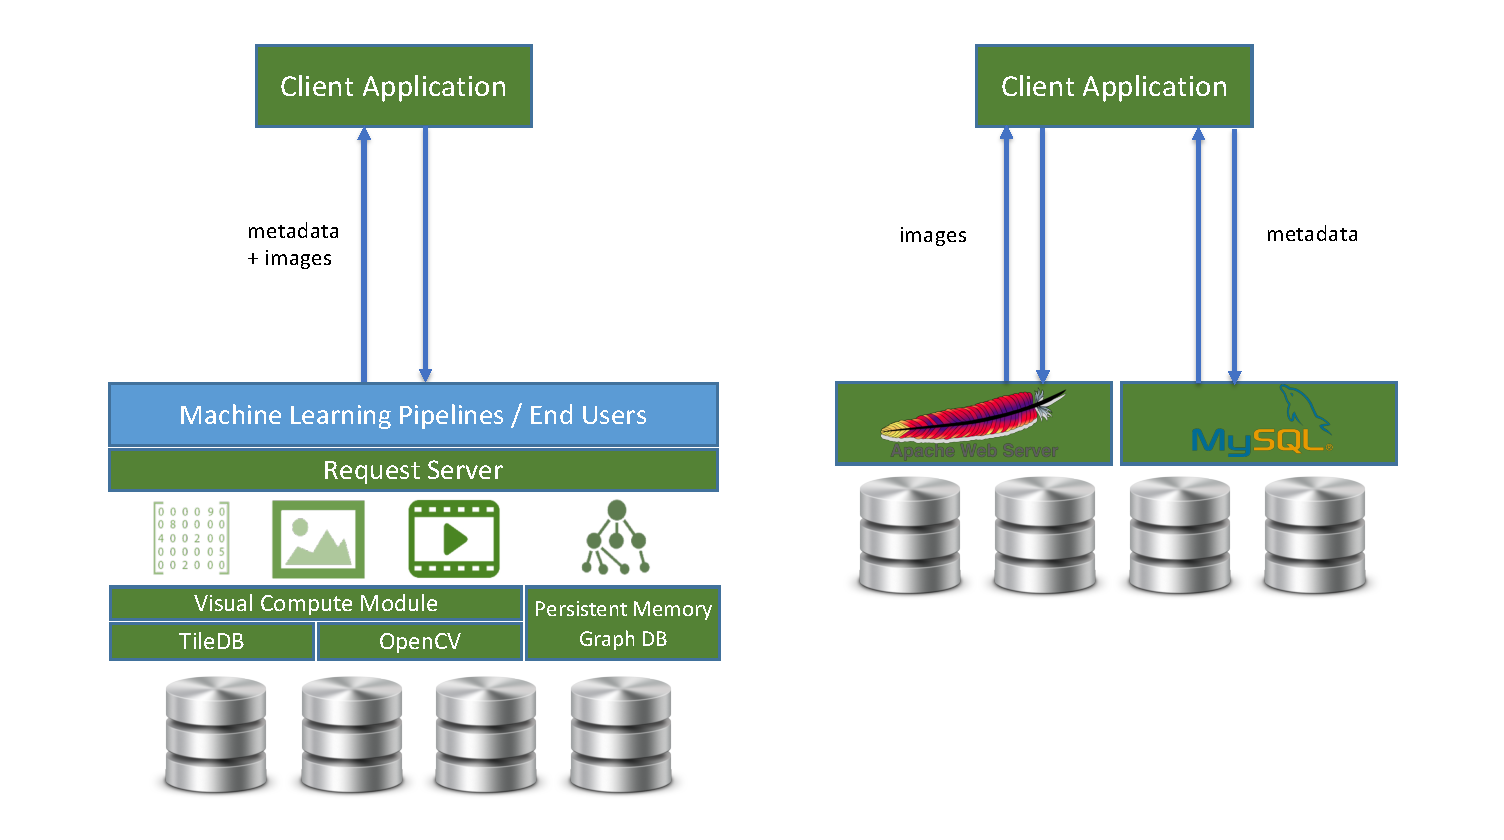
\includegraphics[width=\textwidth]{figures/comparison_system}
\caption{Comparison Systems}
\label{fig:systems}
\end{figure*}

We built VDMS and MySQL databases using the YFCC100M dataset with incremental database sizes 100k, 500k, 1M, 5M, 10M, 50M, and 100M. For each database size, we created a PMGD graph from the YFCC100m metadata, the YFCC100m autotags associated with each metadata identifier, and a list of 1,570 autotags using 100 concurrent VDMS Python clients.  With simple queries, we insert 1,570 nodes for the autotags and insert nodes for the YFCC media objects with the appropriate metadata.  Adding the autotag confidence scores is a recursive process and requires more complex queries than adding the previous nodes. For each metadata identifier in autotags, the query must find the associated metadata node and tag node.  A connection between the two nodes is created with the confidence score as a property. The number of metadata nodes are dependent on the database size and the connections are responsible for 90\% of the elements in each database as shown in Table~\ref{table:vdmsnodes}. It is important to note that the metadata identifier, autotags, and longitude/latitude coordinates are set as indexes of the database to allow faster retrieval of the metadata.

\begin{table}[h]
\caption{Nodes in VDMS database}
\centering
\begin{tabular}{c c c c}
\hline\hline
Database Size & Connections & Images & Autotags\\
\hline
100k & 848,432      & 100,000     & 1,570\\
500k & 4,249,500    & 500,000     & 1,570\\
1M   & 8,503,045    & 1,000,000   & 1,570\\
5M   & 42,505,478   & 5,000,000   & 1,570\\
10M  & 85,040,404   & 10,000,000  & 1,570\\
50M  & 425,162,070  & 50,000,000  & 1,570\\
100M & 895,572,430  & 99,205,984  & 1,570\\
\hline
\end{tabular}
\label{table:vdmsnodes}
\end{table}

Each MySQL database is created in a similar manner but the data is represented as three tables: taglist, metadata, and autotags.  By default, MySQL uses inifinite number of threads inside InnoDB when processing requests using four threads per IO read/write.  In some cases, when creating large databases data locks may occur to protect the data from concurrent updates.  To minimize locking in our runs, we increased the InnoDB buffer pool size to increase the amount of memory allocated to in-memory data structures ~\cite{mysql,mysql_blog}. Using a Python client and simple queries, the taglist table is read from the list of tags with an auto-incremented tagid as an index and the metadata table is read from the YFCC100m metadata using the identifier as an index. The autotags table contains the generated autotags and confidence scores for metadata entries of the metadata table. To generate the table, we split the autotags data for each database by the metadata identifier and autotag into new files. The new files are read into the respective autotags table with the metadata identifier and tagid as indexes.

\begin{table}[h]
\caption{Rows in MySQL database}
\centering
\begin{tabular}{c c c c}
\hline\hline
 & \multicolumn{3}{c}{Table}\\
\cline{2-4}
Database Size & Autotags & MetaData & Tag List\\
\hline
100k & 848,912     & 100,000    & 1,570\\
500k & 4,241,200   & 498,707    & 1,570\\
1M   & 8,508,380   & 1,000,000  & 1,570\\
5M   & 42,425,905  & 4,987,379  & 1,570\\
10M  & 85,095,265  & 10,000,000 & 1,570\\
50M  & 425,446,208 & 50,000,000 & 1,570\\
100M & 896,002,496 & 99,206,564 & 1,570\\
\hline
\end{tabular}
\label{table:mysqltables}
\end{table}

\begin{figure}[]
\centering
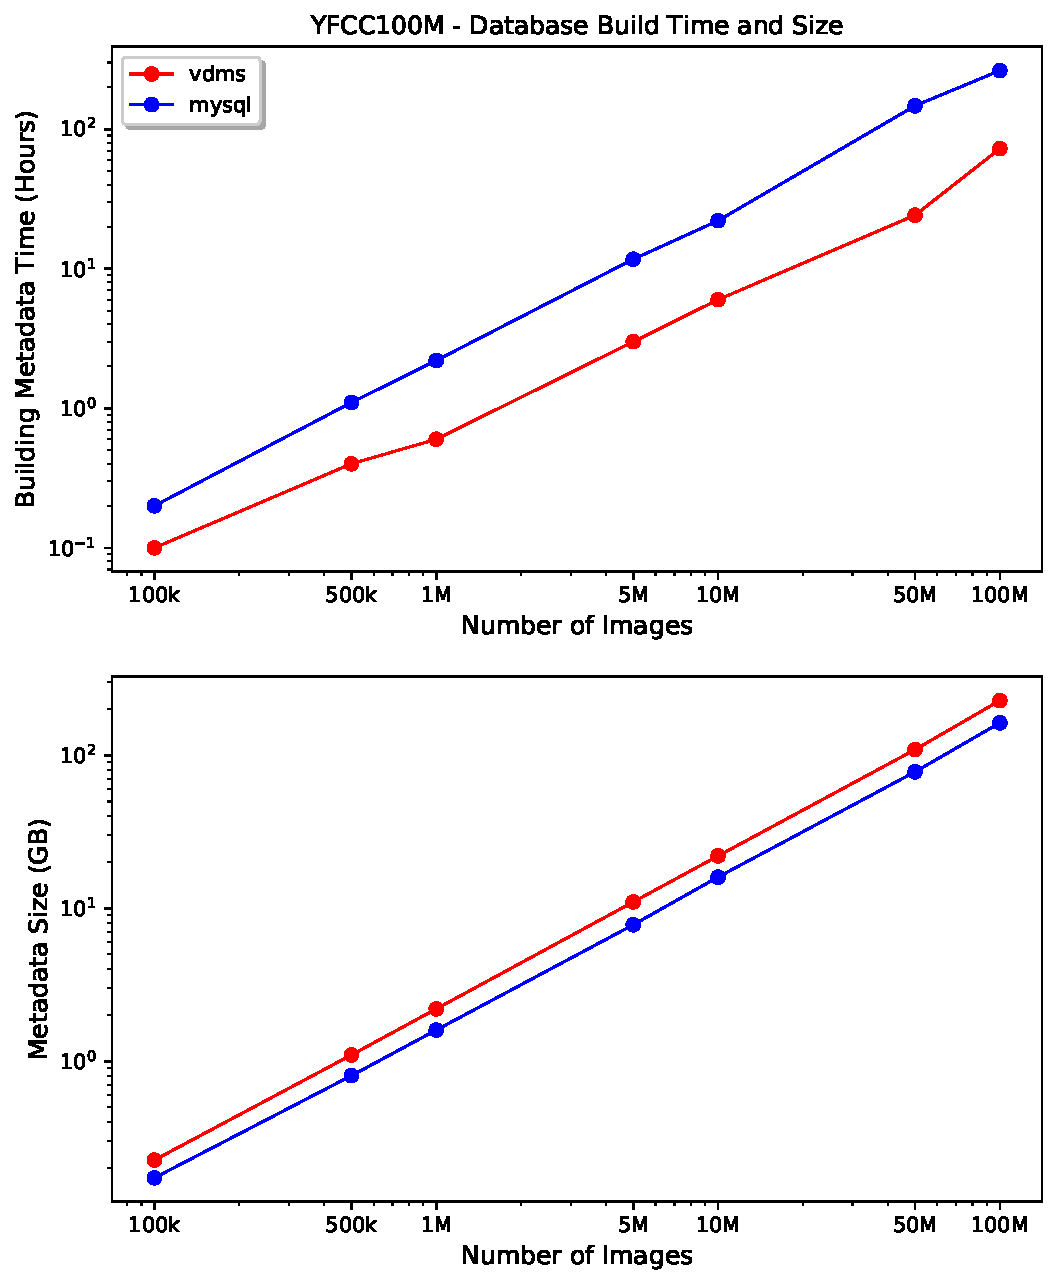
\includegraphics[width=\columnwidth]{figures/db_time_size}
\caption{Time (in hours) to build and size (in GB) of MySQL and VDMS databases}
\label{fig:db_time_size}
\end{figure}

The VDMS and MySQL databases have comparable number of elements as shown in Table~\ref{table:vdmsnodes} and ~\ref{table:mysqltables} but VDMS outperforms MySQL in build speed.  Figure~\ref{fig:db_time_size} illustrates how VDMS can build databases faster than MySQL as the database size grows.  Key difference in the build times are contributed to the low-level implementation of how MySQL reads and stores data from the files and the optimizations (increased InnoDB pool size, etc.) needed to handle large datasets such as YFCC100m.  On average, it took MySQL 3.72x hours longer to build each database than VDMS. For example, to build the 100M database, MySQL took 263 hours while VDMS only needed 72.5 hours.  This is a difference of over 7 days of processing data with VDMS missing less than 0.001\% images and 0.048\% connections from the entire dataset.  Alternatively, VDMS requires more storage, shown in Figure~\ref{fig:db_time_size}, to store information about each node/connection.  This may become a factor if storage is a limitation.  For our runs, VDMS required 30-41\% more storage than MySQL.


\subsection{Images + Metadata}

In order to evaluate VDMS and the baseline on certain queries, we
implement 4 queries that would enable us to retrieve certain specific images.
We choose these queries because they represent typical use-case where a
cohort of images is to be retrieve and processed from a large corpus of data.
We use the metadata associated to the images to filter said images.
In particular, this dataset contains a set of around 1500 machine generated
tags to each image.
Tags includes things like objects (chair, person, people, etc), and
concepts like places (indoor, outdoor, lake) and others (party, etc).
Together with each tag, a probability is assign.
This is, an image can have the tags people, person, party, outdoor, and each
tag will be accompanied by a probability of that tag in that image.
We represent that probability
On average there are 8 tags assigned to each image.
Also, some images have geo-location information (latitude/longitude).

We use the tags (because they contain information about the content of
the image), as well as the geo-location (as an example of searchable properties
of the images).

On top of that, we assume the use case of further processing of images
through the use of ML, such as Convolutional Neural Networks TODO-CITE HERE.
For this, we resize the images to 224x224, which is the input layer size for
a popular neural network for object detection on images: ResNet TODO-CITEHERE.

To evaluate the access to metadata and images,
we use the following four queries:
\begin{enumerate}
\item {\bf {\em 1tag}}: Find metadata/images with 1 specific tag (i.e. alligator, lake, etc).
\item {\bf {\em 1tag\_resize}}: Find metadata/images with 1 specific tag and resize to 224x224.
\item {\bf {\em 1tag\_resize\_geo}}: Find metadata/images with 1 specific tag, resize to 224x224, and in a particular geolocation (with a 20 degrees radius in latitude and longitude).
\item {\bf {\em 2tag\_resize\_geo}}: Find metadata/images with 2 specific tags (i.e. alligator AND lake) and resize to 224x224.
\end{enumerate}

It is important to note that then querying for images with certain tags, we
also apply a filter using the probability. To give an example, we only retrieve
images with a tag "alligator" and a probability higher than 92\%.
This probabilities are both present in VDMS (in the form of metadata present
in the connection between the image and that tag), as well as in MySQL (in
the form of a column of the table that links images with tags).

\begin{figure}[]
\centering
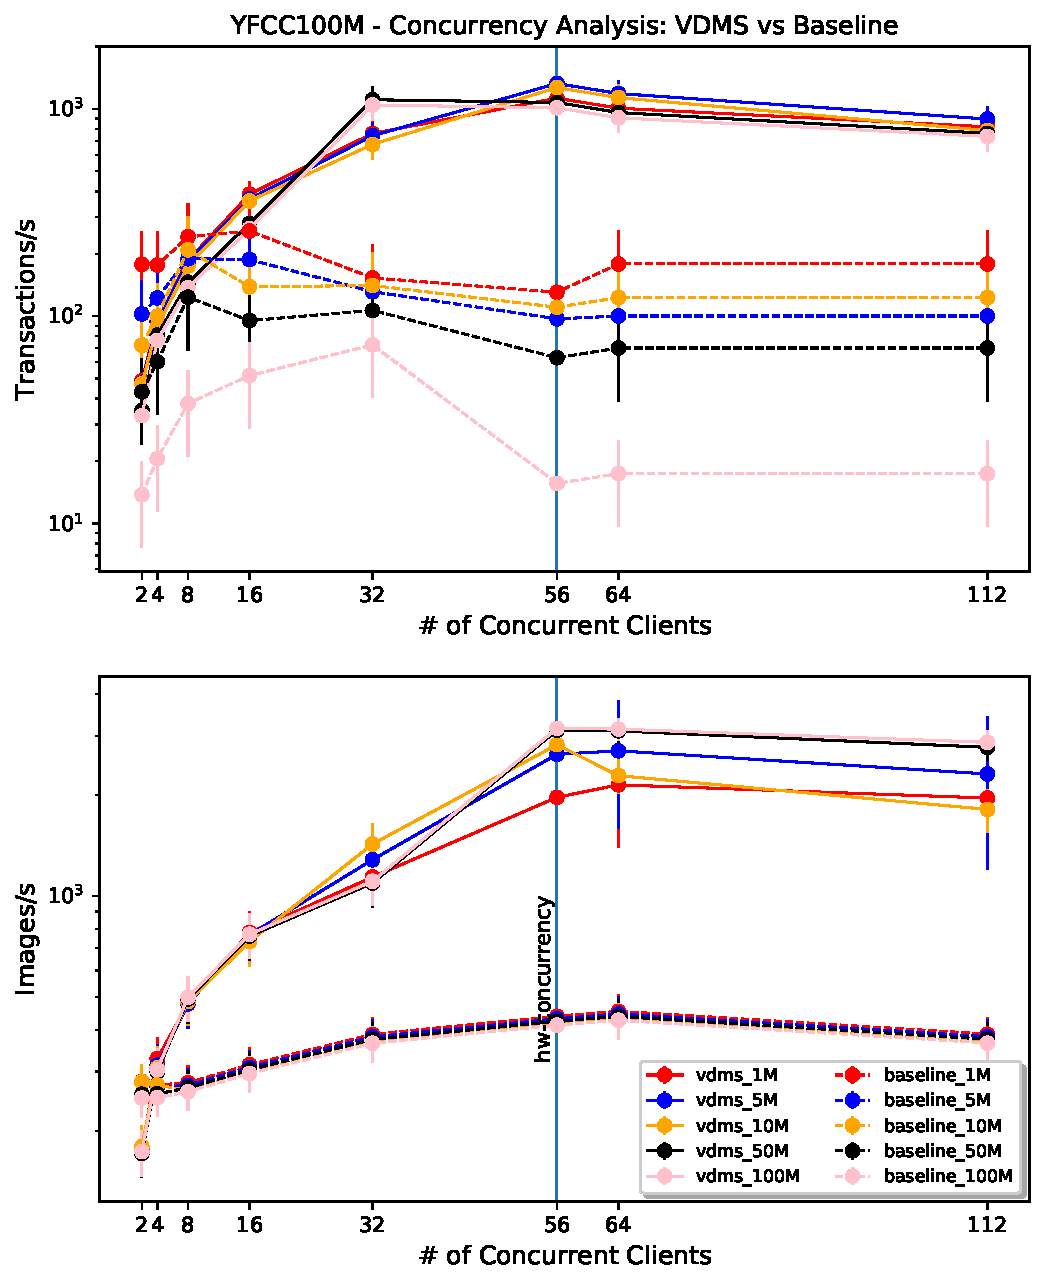
\includegraphics[width=\columnwidth]{figures/concurrency_comparison}
\caption{Concurrency Analysis on Query \"1tag\_resize\"- VDMS vs Baseline}
\label{fig:concurrency_vdms}
\end{figure}



\begin{figure}[t!]
\centering
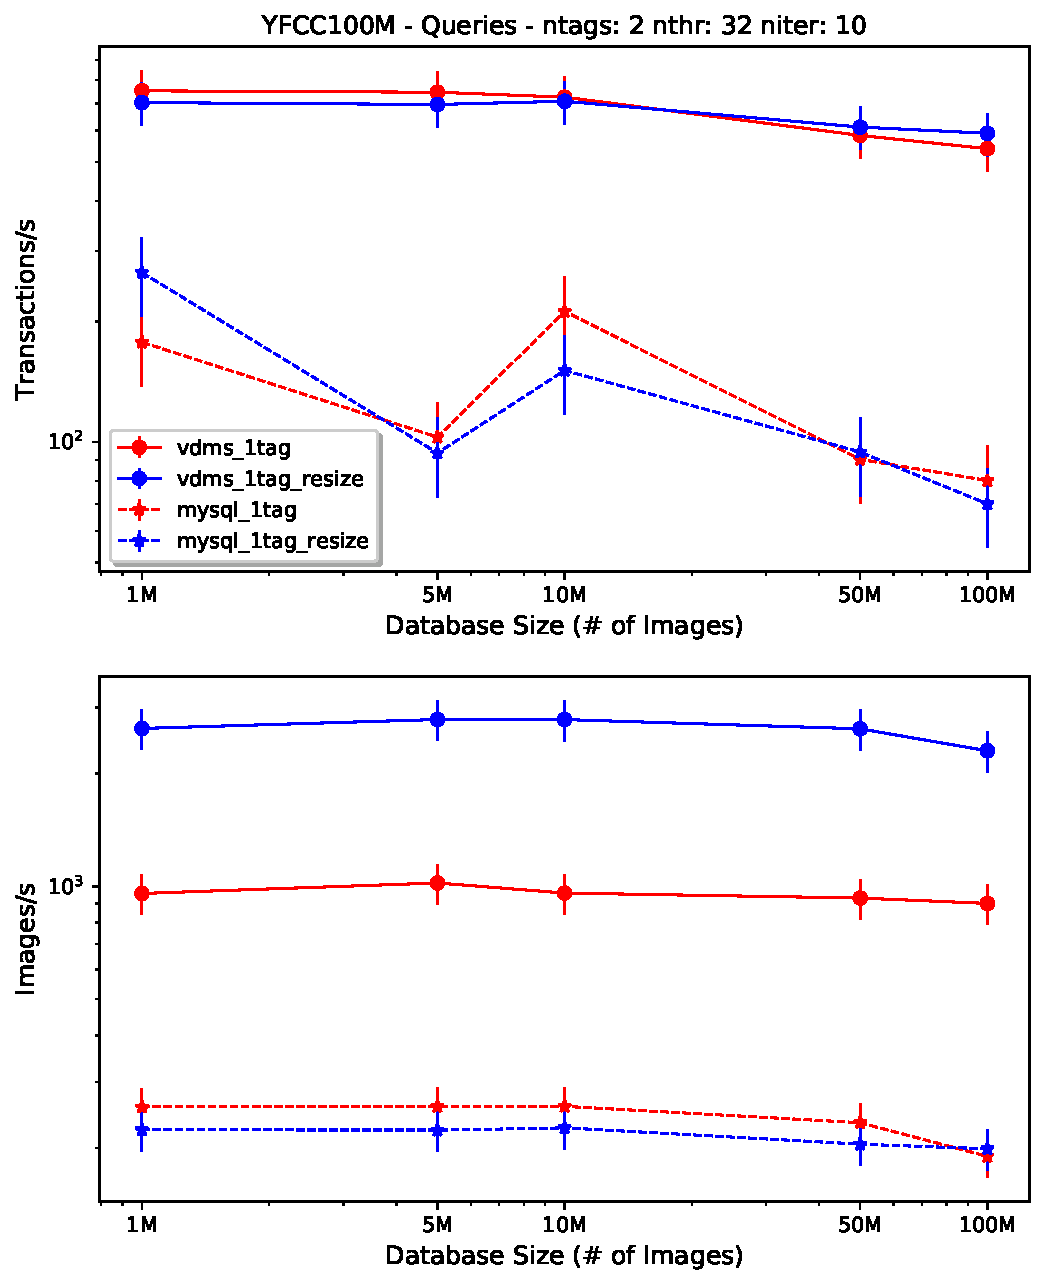
\includegraphics[width=\columnwidth]{figures/queries_throughput_32}
\caption{Queries - Throughput - 32 Clients}
\label{fig:q_throughput_32}
\end{figure}

\begin{figure}[t!]
\centering
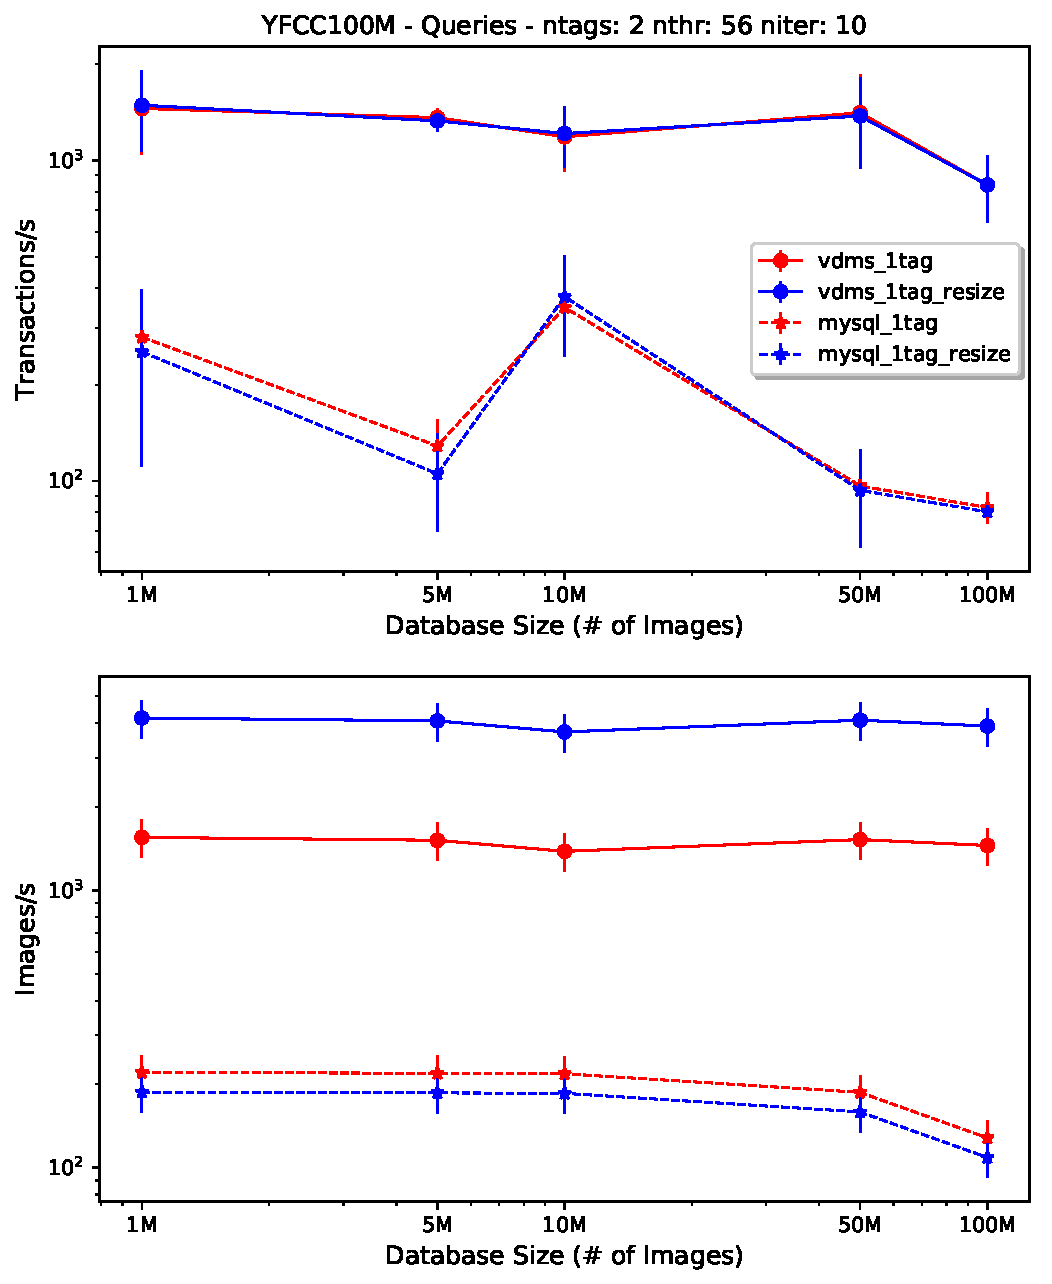
\includegraphics[width=\columnwidth]{figures/queries_throughput_56}
\caption{Queries - Throughput - 56 Clients}
\label{fig:q_throughput_56}
\end{figure}

An image and metadata search on the YFCC100M databases are very extensive
and would benefit from multithreading to process queries simultaneously.
Figure~\ref{fig:concurrency_vdms} illustrates a concurrency analysis for
the \textit{1tag} query using VDMS to investigate the number of
concurrent clients to use for the per-query performance analysis.
This figure shows the metadata performance plateaus at 32 clients and
the image performance at 56 clients for a simple query.
To further investigate, Figure~\ref{fig:q_throughput_32} and
Figure~\ref{fig:q_throughput_56} illustrate the throughput performance
for the \textit{1tag} and \textit{1tag\_resize} queries for 32 and 56 clients,
respectively.
On the 56-client experiment, a 10x difference occurs between VDMS and
MySQL in metadata throughput while 32 clients is similar but not as high.
The overall performance for both MySQL and VDMS is better with 56 clients;
therefore, we used this value for our per-query analysis.

\begin{figure}[]
\centering
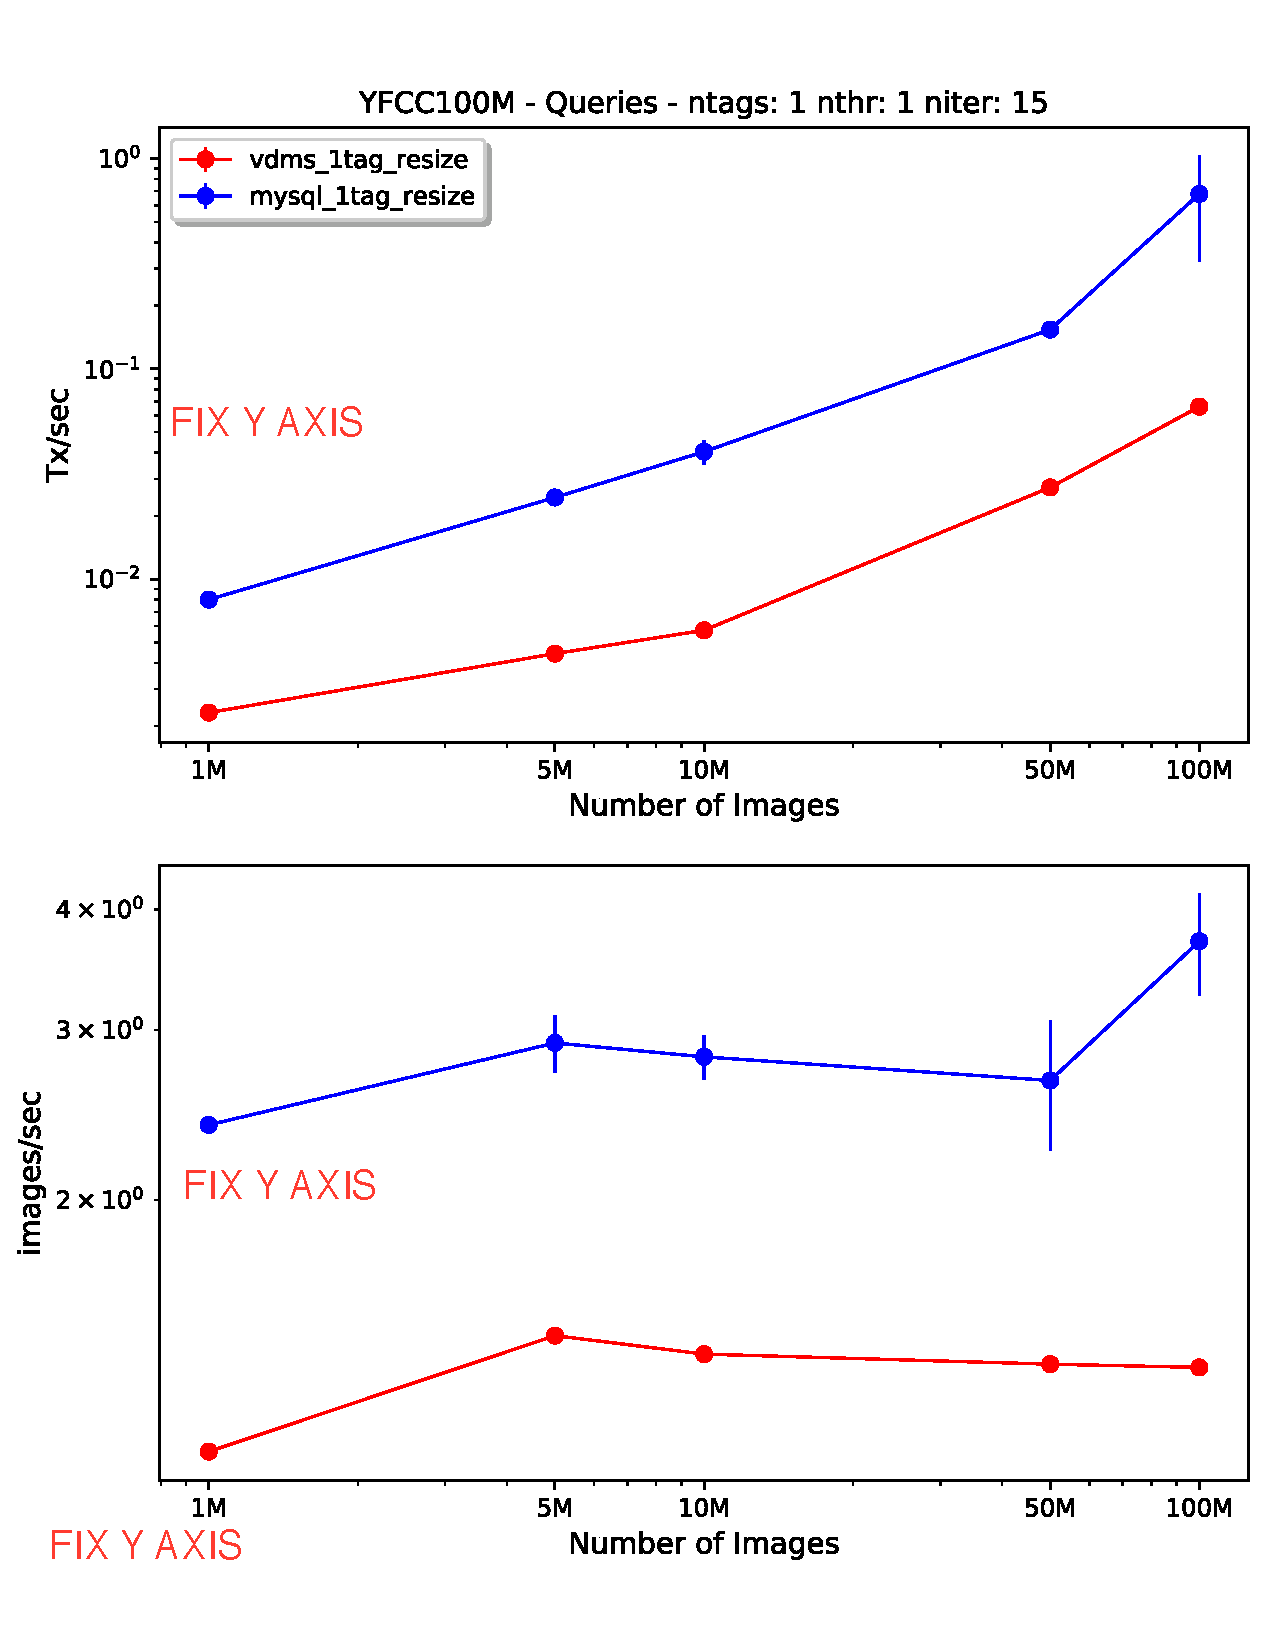
\includegraphics[width=\columnwidth]{figures/q1_latency}
\caption{Query 1 - Latency}
\label{fig:q1_latency}
\end{figure}

\subsection{Videos}

\begin{figure*}[ht!]
\centering
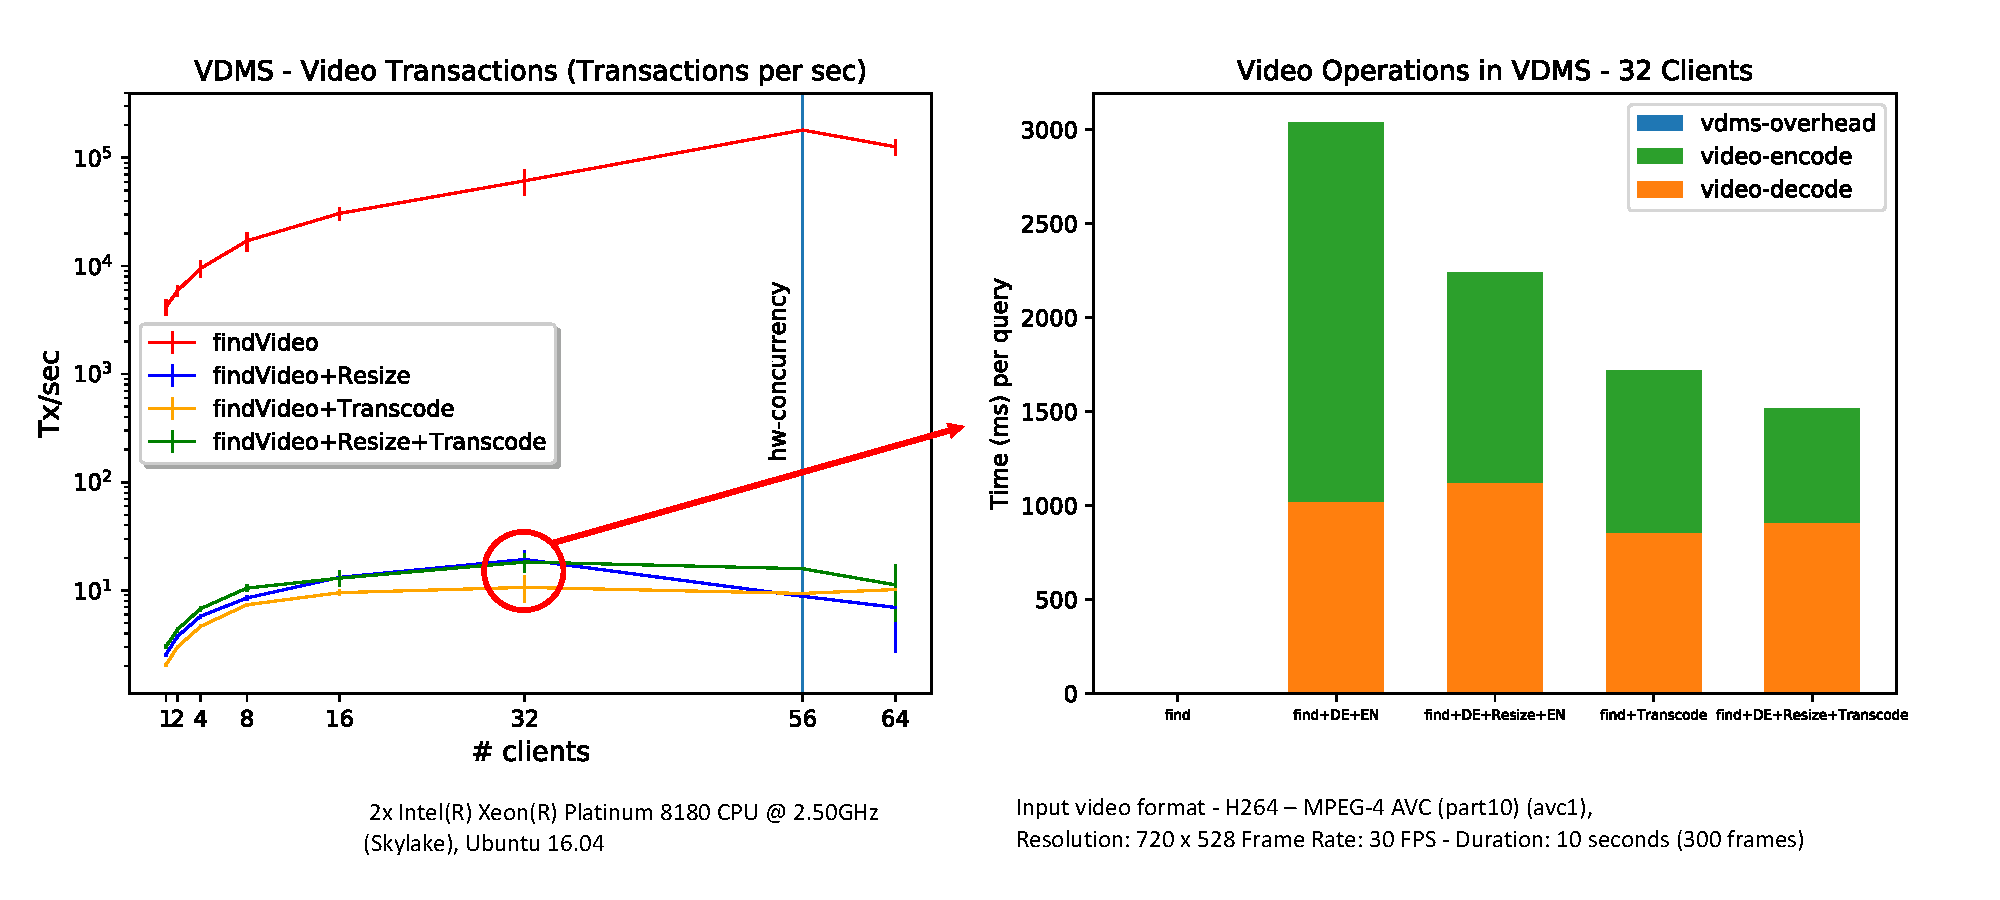
\includegraphics[width=\textwidth]{figures/video_overhead}
\caption{Concurrency (left) and Overhead (right)}
\label{fig:video}
\end{figure*}

VDMS provides full support for video storage and operations.
This includes support for encoding/decoding and trans-coding of mp4, avi, and
mov containers, as well as support for xvid, H.263 and H.264 encoders.
This is supported through the Visual Compute Module that provides an abstraction
layer on top of OpenCV (and ffmpeg directly).
All the operations supported for images in VDMS are also supported at the
video and frame level on the API. On top of that, there are a number of
video-specific operations that are supported, such as the interval operations,
that allow users to retrieve clips at different FPS versions of the video.

All this functionality is provided and integrated with the rest of the
metadata API as part of the comprehensive VDMS interface. This makes it
possible for users to interact with metadata and video in a transactional
manner, enabling users to run queries like: "Retrieve all the videos
where there is a lake with probability higher than X, converting all videos
to H.264 mp4 of size 224x244".
In particular, this functionality was used internally to select a subset
of videos with the right licenses for a video summarization application.

To the best of our knowledge, there is no solution that can provide
all the functionality mentioned above. Also, implementing a baseline is a very
complex task as there is a large number of options and parameters that can
be chosen, which makes it hard to accurately compare against VDMS functionality.
For this reason, we chose to make a study using VDMS in various scenarios,
and analysis what is the impact of having the overhead of VDMS' Request
Server in the overall access time.

Figure \ref{fig:video} shows the analysis of different queries aimed to retrieve
a video using VDMS interface. We show how VDMS increases throughput of serving
a video object as the number of simultaneous client increases, as well as the
overhead VDMS introduces in the overall query execution time.
The figure on the left compares the number of video transaction per second
(i.e., number of videos returned per second) when different operations
are executed as part of the transaction. The upper-bound of this would be
simply returning the video as-is (without running any encoding/decoding or
operation), represented by the red line. This query is the upper-limit because
it essentially translates to reading the video from the file-system and sending
it over a TCP/IP socket, without any other overhead or operations.

We also run a set of other queries that involve: (a) running a resize operation
on the video and, consequently, needs a decoding and
encoding operations as well (blue line),
(b) transcoding, meaning the use a different container and encoder
than the one originally used (yellow line), and (c) both resize and transcoding.
Note that the resize operation performs a downsize, which translates in less
data being sent over the wire. This is specially noticeable when supporting 32
simultaneous clients, where the systems provides more videos per second due to
sending less data to the client, when compares to just transcoding and not resizing (yellow line).

We can see that the system performs best when using all the physical cores.
COMPLETE THIS BETTER.

WE SHOULD ADD HERE SAMPLES OF THE QUERYS TO SHOW HOW THESE ARE RETRIEVED.

Because we see almost 3 orders of magnitude drop in performance when including
operations as part of the query, we wanted to understand where most of the time
was spent on the query, and optimize the Request Server and Visual Compute Module
if necessary. For this, we run the experiment shown at
Figure \ref{fig:video} (right) which breaks down the different components of the
queries. This figure shows that more than 97\% of the query execution is spent
on encoding/decoding operations, which is well-known to be a
heavy and compute intensive operation.
On the one hand, this results show that VDMS introduced overhead for
video operation is minimal. On the other hand, this result means a
limit on the opportunities for optimization for video queries given
that biggest time factors are accounted by encoding/decoding, which is
outside the scope of VDMS.
This result also was the inspiration point for one optimization we included
in future versions of VDMS, which involves using ffmpeg C++ API to
limit the number of frames being encoding/decoding when possible.


\subsection{Feature Vectors}

Another key differentiating factor of VDMS is that it allows the creation of
indexes for high-dimensional feature vectors and the insertion of
these feature vectors associated with entities or visual objects.
Feature vectors are intermediate results of various machine
learning or computer vision algorithms when run on visual data.
Feature vectors are also known as "descriptors" or "visual descriptors".
We use these terms interchangeably.
These descriptors can be labeled and classified to build search indexes,
and there are many in-memory libraries that are designed for
this task~\cite{flann, faiss}.
Using the VDMS API, users can manage feature vector indexes,
query previously inserted elements (images),
run a k-nearest neighbor search (knn) and express relationships
between existing images or descriptors and
the newly inserted descriptors.
By natively supporting descriptors and knn,
VDMS allows out-of-the-box classification
functionalities for many applications.

For this work, and as part of a comprehensive image search implementation,
we have used 4096-dimensional descriptors extracted from every image
(and first frame of every video) and created a collection of these feature
vectors in VDMS to be able to perform similarity search (i.e., find
images that are "similar" to an query (input) image).
"Similarity" in this particular case is defined as closeness
in a an 4096-dimensional space using euclidean distance as the metric.

EXPLAIN HERE DIFFERENT ACCURACY/EXECUTIME TIME TRADEOFF.

The process of loading descriptors in VDMS is simple.
First, the user has to create a DescriptorsSet, using a single command.
At creation of the DescriptorSet, the dimensionality of the descriptors
is specified, together with the desired indexing method and the desired metric
for computing distances (Euclidean Distance, L2, or Inner Product, IP).
Once the DescriptorSet is created, descriptors can be inserted to the set.
After the descriptors are inserted, similarity search can be performed.
Note that descriptors can be inserted later on, and any search will reflect
the existence of all descriptors in the set.

\begin{figure*}[]
\centering
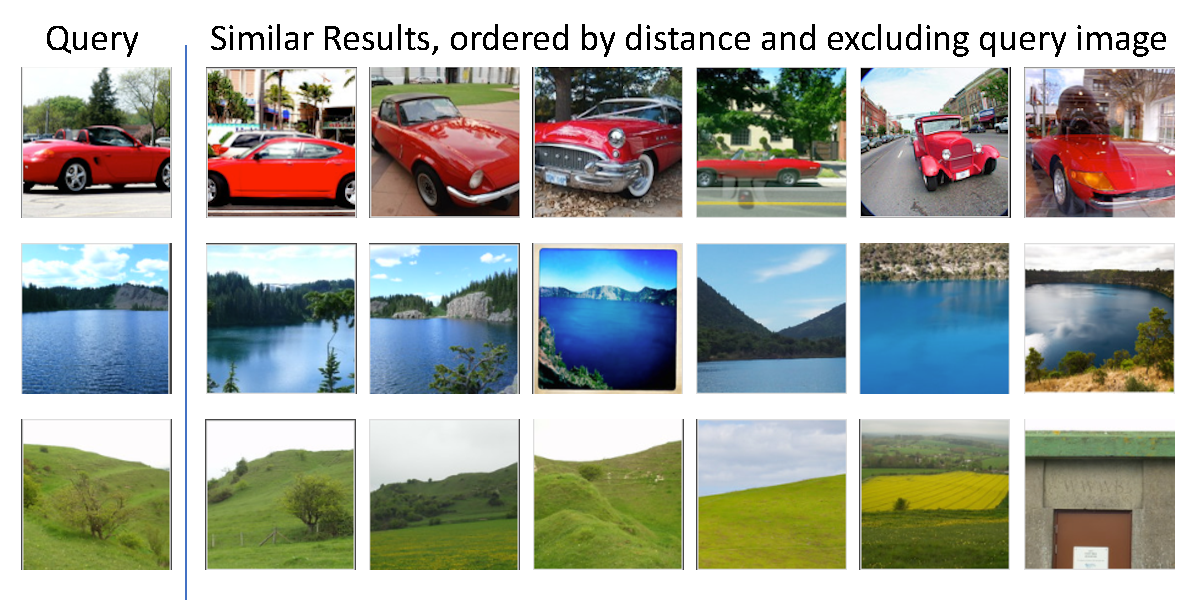
\includegraphics[width=\textwidth]{figures/feature_img_results}
\caption{Sample Results of Similarity Search}
\label{fig:similarity}
\end{figure*}

Figure \ref{fig:similarity} shows 3 examples of a query image (on the left),
and images returned as "similar" by VDMS.
The query input is a descriptor generated after a query image. The "query"
descriptor is sent to VDMS as part of the query, and VDMS use that descriptor
to find similar one, and retrieve the images associated with those "similar"
descriptors. We used this as an example and as a visual validation of the
functionality and applicability in this particular dataset, but we also
provide an analytical approach to accuracy and trade-offs in our system.
It is important to note that the accuracy of the results is entirely tied
to the quality of the descriptors chosen by the applications.
VDMS is completely agnostic to information contained within the descriptor,
and simply offers the interface to store and index them, but the quality
of the similarity result will be tied to the quality of descriptor extraction
that the application is using.


\begin{figure*}[]
\centering
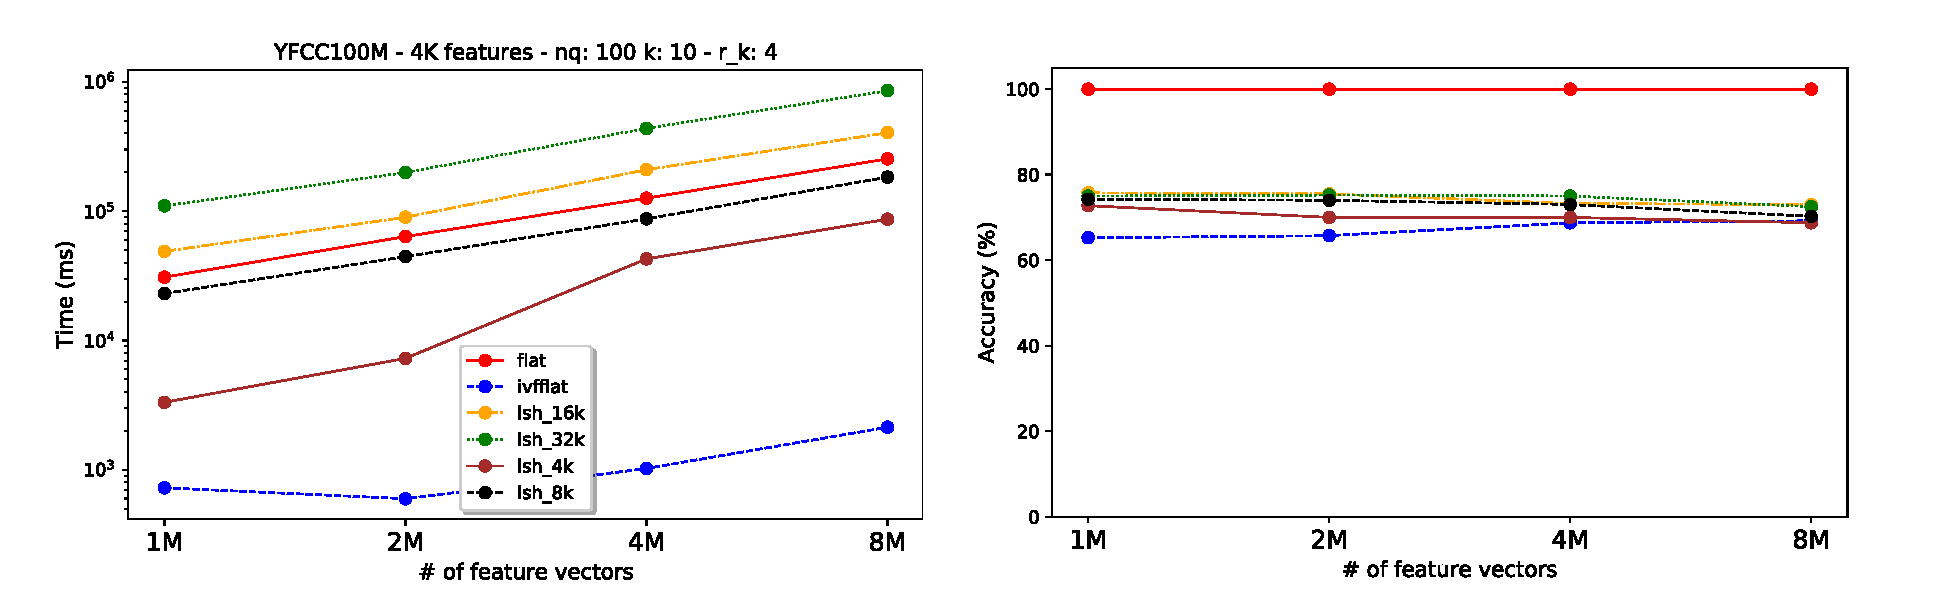
\includegraphics[width=\textwidth]{figures/features_alternatives}
\caption{Feature Vector Evaluation: Trade-off between query execution speed
and accuracy of the results, using ground-truth data for computing accuracy.
For this evaluation, we query the 10 closest neighbors (k = 10), and compute
accuracy using recall at 4 (r\_k = 4) (i.e. percentage of the top 4 ground-truth
results that is present within the top 10 computed neighbors).
We average the query execution time and accuracy for 100 queries (nq = 100).}
\label{fig:features_eval}
\end{figure*}

As mentioned before, VDMS provides different levels of customization of the
indexes created for a descriptor set, that includes the indexing techniques
and the metric for similarity.
These different indexing techniques comes with different trade-offs in terms
of speed of search and accuracy.
VDMS aims to provide functionality that is agnostics to application-specific
techniques, enabling functionality that is general to visual data processing
applications.
Figure \ref{fig:features_eval} shows an analysis at the different indexing
techniques provided by VDMS and its trade-off between accuracy and query
execution speed, for a single threaded client.
For this evaluation, we query the 10 closest neighbors (k = 10), and compute
accuracy using recall at 4 (r\_k = 4) (i.e. percentage of the top 4 ground-truth
results that is present within the top 10 computed neighbors).
We average the query execution time and accuracy for 100 queries (nq = 100).
The "flat" index (red line) implements exact search and
represents ground-truth, which explain why the accuracy is always 100\% on the
right plot. The other indexes implement "approximate search", which trade-offs
between accuracy and speed of search~\cite{flann, faiss}.
We have also tried the "ivfflat" index (inverted file index), as well as
LSH-based indexes using a different number of bits per descriptor.
\footnote{https://github.com/facebookresearch/faiss/wiki/Faiss-indexes}.
Results show how "ivfflat" is the fastest option by comes at the trade-off
of about 30\% lost in accuracy, while simple brute-force search
is among the slowest options at the expenses of 100\% accuracy,
meaning exact search.

\begin{figure*}[]
\centering
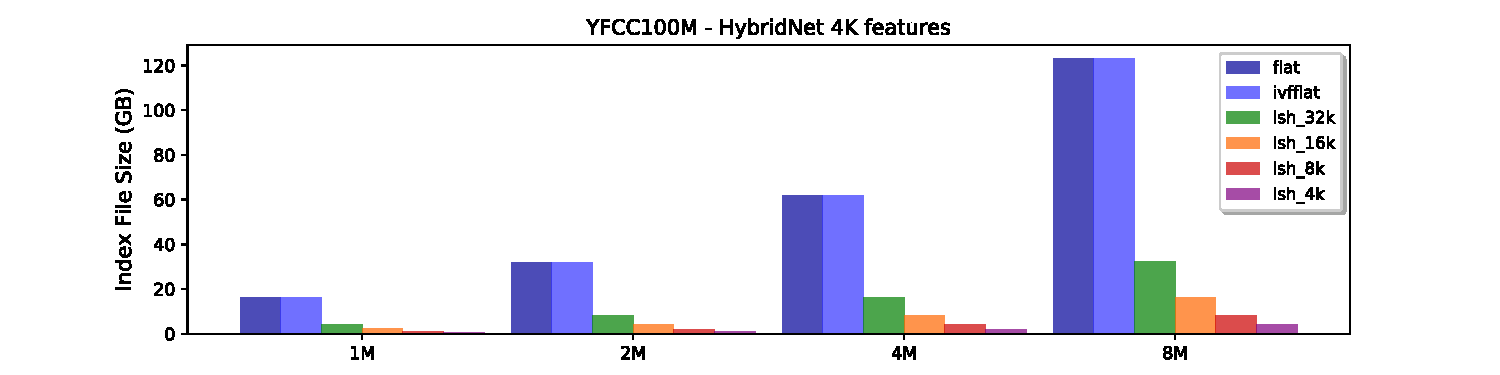
\includegraphics[width=\textwidth]{figures/features_disksize}
\caption{Feature Collection Size in Disk}
\label{fig:features_size_does_matter}
\end{figure*}

Another important trade-off to be made is w.r.t to space efficiency: Set of
descriptors can grow very large and hard to manage.
In this particular case, 4096-dimensional descriptors for 100M elements
translates into 1TB of data, only in raw floating-point data alone (without
accounting for any metadata or indexes associated with it).
This component is very important on the overall analysis because a large set
of feature vectors may not fit in memory and thus cause a pressure on the IO
system while retrieving descriptors for computing distance, that severely impact
the overall query execution time.
Because of this, when the set of descriptors grows significantly large,
it may be worth trading off accuracy to speed and space.
Figure \ref{fig:features_size_does_matter} show the different indexes and
their size in disk. These indexes already contain all the descriptors (or
a quantized version of them), and can be loaded in memory directly when it fits.
Note how, because of quantization of the descriptors,
LSH provides a significantly lower space foot print, which can be a great option
for large collections of descriptors when accuracy is not a main factor.

